\chapter{Reducing quantum fluctuations with squeezed light}\label{ch:squeezed}

The precision of a beam deflection measurement is limited both by fundamental sources of uncertainty derived from quantum mechanical considerations, as well as unavoidable sources of technical noise present in any laboratory setting.  

The possibility of reducing the quantum uncertainty of an observable using squeezed states of light was recognized in the early 80s.  In a particularly significant paper along these lines, Caves~\cite{Caves1981} showed that the precision of interferometric phase measurements could be improved by using squeezed states to reduce quantum vacuum fluctuations.  Precision phase measurements beyond the so-called ``shot-noise limit'' or ``standard quantum limit'' were experimentally realized later in the decade \cite{Xiao1987} with the generation of sufficiently strong squeezed light using optical parametric amplifiers (OPAs).  This technique was extended both theoretically and experimentally later to improve the sensitivity of beam deflection measurements \citep{Treps2002,Treps2003}.

The separate technique of weak value amplification was introduced theoretically in 1988 by Aharonov, Albert, and Vaidman \cite{Aharonov1988}, and observed in optical beam measurements later \cite{Hosten2008,Dixon2009,Starling2009,Starling2010}.  For precision measurements, it has been shown~\cite{Starling2009} that the principle advantage weak value amplification has over competing techniques lies in the significant reduction in technical noise due to the ``post-selection'' process which allows only a small fraction of input photons to reach the detector with an amplified deflection signal.

Using both squeezed light and weak value amplification in concert allows us to simultaneously reduce the quantum uncertainty of the transverse position observable and technical noise encountered in the lab.  
\section{Squeezed Weak Value Measurement}
\begin{figure}
  \begin{center}
    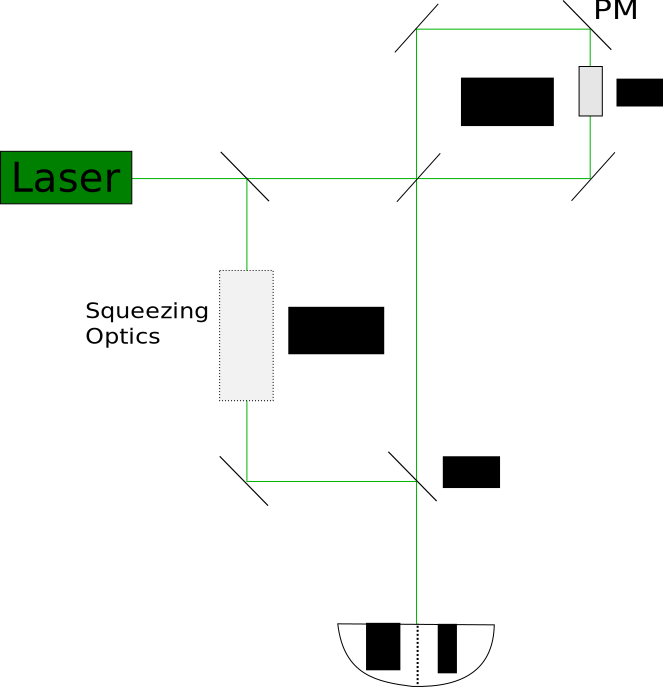
\includegraphics[width=\columnwidth]{./SqueezedLight/figures/basic_experiment}
  \end{center}
  \caption{Basic setup for reducing the quantum noise of a weak value amplification measurement using squeezed light.  Coherent light from the laser is split into two beams- one travels through the Rochester setup WV interferometer (Int 1) with deflection-amplified photons leaving the dark port, the other travels through ``squeezing optics'' which create a flipped mode in a squeezed vacuum state as in \cite{Treps2002,Treps2003} in Int 2.  The beams are combined using a highly reflective beamsplitter (BS) ($R > 90\%$) and are then incident on a split detector. }  
  \label{fig:setup}
\end{figure}
%\begin{figure*}
%  \begin{center}
%    \includegraphics[width=6in]{./figures/sagnac_out.pdf}
%  \end{center}
%  \caption{Output mode of the Sagnac interferometer with $\phi = \pi/16$.  In both plots the blue curve represents $\ell = 1\text{m}$ (a 2m interferometer) and the red dashed curve represents $\ell = .25\text{m}$.   Left: The real part of the Sagnac output transverse wavefunction.  Right: The imaginary part.  }  
%  \label{fig:sagnacoutput}
%\end{figure*}
Using the basic configuration shown in Fig.~\ref{fig:setup}, we may combine the output of the dark port of a Rochester setup weak-value measurement with squeezed vacuum states. Coherent light prepared in a Gaussian mode from the laser is deflected by the piezo-mirror in the Sagnac interferometer.  The squeezed light source creates a squeezed vacuum prepared in a ``flipped'' Gaussian mode described below.  Though the coherent mode is deflected and the squeezed mode is not, this will only trivially affect the measurement provided the beam deflection is small compared to the beam width.     

The effect of squeezed light on split-detected beam deflection measurements has been theoretically examined in detail by Barnett et al.\ in Ref.~\cite{Barnett2003}.  In that paper, they consider both coherent and squeezed vacuum states of light.

The coherent state $\ket{\alpha}$ can be written with the help of the displacement operator $\op{D}(\alpha) = \exp(\alpha \creation{a}{} - \alpha^{*} \annihilation{a}{})$ as
\begin{align}\label{eq:displacementop}
\ket{\alpha} = \op{D}(\alpha) \ket{0},
\end{align}
where $\ket{0}$ is the vacuum state.  The complex number $\alpha$ satisfies the eigenvalue equation $\op{a}\ket{\alpha} = \alpha\ket{\alpha}$ and hence the average number of photons in a coherent state is given by $\bra{\alpha}\numberop{a}{}\ket{\alpha} = |\alpha |^2$.

The squeezed vacuum state $\ket{\zeta}$ can be obtained in a similar manner by using the ``squeeze operator'' $\op{S}(\zeta) = \exp(\frac{1}{2}(\zeta^{*}\annihilation{a}{}^2 - \zeta \op{a}^{\dagger\: 2}))$,
\begin{align}
\ket{\zeta} = \op{S}(\zeta)\ket{0}.
\end{align}
Writing the complex squeeze parameter as $\zeta = re^{i\nu}$, the average number of photons in a squeezed vacuum state is given by $\bra{\zeta}\numberop{a}{}\ket{\zeta} = \sinh^2 r$.

Using the Gaussian and ``flipped'' modes given by
\begin{align}
\nonumber u_0(x) &= \frac{1}{\sqrt{\pi^{1/2}\sigma}}e^{-x^2/2\sigma^2},\\
u_1(x) &= \frac{1}{\sqrt{\pi^{1/2}\sigma}}e^{-x^2/2\sigma^2}\text{sign}(x),
\end{align}
it is possible to beat the standard quantum limit by using squeezed light to reduce noise due to vacuum fluctuations.  If the $u_0$ mode is prepared in a coherent state and the $u_1$ mode is prepared as a squeezed vacuum then the variance in photon counts between the two sides of a split detector is 
\begin{align}\label{eq:generalvariance}
\nonumber\mathcal{N}^2 = \sinh^2 r +& |\alpha |^2[\cosh 2r \\
&- 2\cos(2\theta - \nu)\sinh r \cosh r ],
\end{align}
where $\theta = \text{arg}\; \alpha$.  The variance is a function of relative phase between the two modes, and takes on its minimum value for $\theta = \nu/2$.  The split-detected signal is given by 
\begin{align}
\mathcal{S} = \frac{2|\alpha|^2 d}{\pi^{1/2}\sigma},
\end{align}
where $d$ is the deflection distance.

For the optimal relative phase between the coherent and squeezed beams the SNR of a displacement measurement is then
\begin{align}\label{eq:squeezedsnr}
\text{SNR} = \frac{2|\alpha |^2 d}{\pi^{1/2}\sigma (|\alpha |^2 e^{-2r} + \sinh^2 r)^{1/2}}.
\end{align}  


From Eq.~\eqref{eq:squeezedsnr} we see that for moderate squeezing ($\sinh^2 r \ll |\alpha |^2$) 
\begin{align}
\text{SNR} = \frac{2d\sqrt{|\alpha |^2} }{\pi^{1/2}\sigma e^{-r}},
\end{align}
which represents an improvement in SNR by a factor of $e^r$ over the standard quantum limit.  Minimizing the denominator of Eq.~\eqref{eq:squeezedsnr} reveals that maximal squeezing can be achieved with the choice $r \approx \text{ln}(4|\alpha |^2)/4$, or equivalently, $\sinh^2 r \approx \sqrt{|\alpha |^2}/2$. For maximal squeezing, the SNR scales as 
\begin{align}
\text{SNR} = \frac{2\sqrt{2}d(|\alpha |^2)^{3/4} }{\pi^{1/2}},
\end{align}
which improves SNR scaling by a factor of $(|\alpha |^2)^{1/4}$.
\subsection{Dark Port Output}

To ensure the analysis from Ref.~\cite{Barnett2003} holds, we must verify that the output of the dark port of the interferometer is a coherent beam in the Gaussian $u_0$ mode.  

For the longitudinal mode, it is straightforward to show that when the appropriate operating point for the SBC is chosen such that $\phi = 0$ corresponds to perfectly bright and dark ports the relevant annihilation operator is given by
\begin{align}\label{eq:darkannihilation}
\annihilation{a}{dark} = \sin\left(\frac{\phi}{2}\right)\annihilation{a}{in} .  
\end{align}
Hence, the annihilation operators describing the dark port output and WV interferometer input only differ by a factor.  This does not modify the form of Eq.~\eqref{eq:displacementop}, so a coherent input beam will yield a coherent output beam.  Note that taking the adjoint of Eq.~\eqref{eq:darkannihilation} and relating the number operators for the input and dark port output correctly recovers the post-selection probability $P_{ps} = \sin^2 (\phi/2)$.

To verify the Gaussian shape of the dark port transverse mode, we examine the effect of our weak measurement on the beam profile.  We consider the ``system'' state $\ket{\psi}$ which describes the path of photons in the WV interferometer and the ``meter'' state $\ket{\varphi}$ describing the transverse beam.  The overall state is then given by the tensor product $\ket{\Psi} = \ket{\psi}\ket{\varphi}$.

With kets $\ket{\cw}$ and $\ket{\ccw}$ describing clockwise and counterclockwise travel in the interferometer, we take the input state to be $\ket{\psi_+} = \frac{1}{\sqrt{2}}\left(\ket{\cw} + i\ket{\ccw}\right)$.  The system state describing post-selection is the the orthogonal $\ket{\psi_-} = \frac{1}{\sqrt{2}}\left(\ket{\cw} - i\ket{\ccw}\right)$.  It is also convenient to introduce the which-path operator $\op{W} = \pr{\cw} - \pr{\ccw}$. 

While traversing the WV interferometer photons will experience two distinct effects, a transverse momentum shift due to the piezo mirror and a phase shift due to the SBC.  The momentum shift is described by the unitary operator $\op{U}_{PM} = e^{-ik\op{x}\op{W}}$ and the phase shift is described by the unitary operator $\op{U}_{SBC} = e^{i\phi\op{W}/2}$.  Post-selected photons are then described by the state $\ket{\Psi_{-}} = \left(\op{M}_{-}\ket{\varphi}\right)\ket{\psi_-}$, with $\op{M}_- = \bra{\psi_-}\op{U}_{PM}\op{U}_{SBC}\ket{\psi_+} = i\sin(\phi/2 - k\op{x})$.

Taking the input of the WV interferometer to be in the zeroth mode of the basis $u_0(x)$, we are able to calculate the dark port profile $\ipr{x}{\varphi}$ as 
\begin{align}
\nonumber \ipr{x}{\varphi} &= \bra{x}\op{M_-}\ket{\varphi_0},\\
&= A\sin(\phi/2 - k x)u_0(x),
\end{align}
where $\ket{\varphi_0}$ is the input state and
\begin{align} 
A = \sqrt{\frac{2}{1-e^{-k^2\sigma^2}\cos \phi}}
\end{align}
is a normalization constant.  The projection of the WV output state on to the initial state is then 
\begin{align}
\nonumber \ipr{\varphi_0}{\varphi} &= A\int \text{d}x\; u_0(x)^2 \sin(\phi/2 - k x), \\
\nonumber &= \sqrt{\frac{2e^{-\frac{1}{2}k^2\sigma^2}\sin^2 \phi/2}{1 - e^{-k^2\sigma^2}\cos\phi}}, \\
&\approx \sqrt{\frac{2\sin^2 \phi/2}{1 - \cos\phi}} = 1.
\end{align}
For our purposes a reasonable upper bound on $k\sigma$ is given by $k\sigma < 10^{-4}$ or equivalently, $k^2\sigma^2 < 10^{-8}$, hence our approximation $e^{k^2\sigma^2} \approx 1$ is valid for all parameters of experimental interest.  Any deviations from a pure $u_0(x)$ mode due to the WV measurement are therefore negligible. 

%We may also include diffraction by introducing the unitary operator $\op{U}_\ell = e^{-i\op{p}^2\ell/2k_0}$, where $\ell$ is the distance traveled by the beam.  Approximating the distance from the laser to the piezo mirror to be equal to the distance from the piezo mirror to the detector to be equal, we may write our modified state as 
%\begin{align}
%\nonumber \ipr{x}{\varphi} &= \bra{x}\op{U}_\ell\op{M_-}\op{U}_\ell\ket{\varphi_0}.
%\end{align}
%
%Setting $k = 0$ we are able to calculate the amplitude of the state leaving the dark port straightforwardly as
%\begin{align}\label{eq:sagnacoutputmode}
%\nonumber \ipr{x}{\Psi} &= \bra{x}\op{U}_\ell \op{M}_- \op{U}_\ell \ket{\varphi}, \\
%\nonumber &= \frac{i \sqrt{\sigma}}{\pi^{1/4}} \sqrt{\frac{k_0}{2i\ell + k_0 \sigma^2}}\text{exp}\left(\frac{k_0 x^2}{4i \ell + 2k_0\sigma^2} \right), \\
%&\equiv \frac{i}{\beta}\sqrt{\frac{\sigma}{\pi^{1/2}}}e^{-x^2/2\beta^2}.
%\end{align}
%
%Here the input of the interferometer is taken to be in the zeroth mode of the basis,
%\begin{align}
%\ipr{x}{\varphi} = u_0.
%\end{align} 
%
%The output mode is still an even function, but has a slightly modified shape from our input Gaussian mode.  If we take $k_0\sigma^2 \gg 4i\ell$ then $\beta \approx \sigma$ and the output of the dark port is simply our $v_0$ basis mode scaled by a complex factor.  In this limit the above analysis holds without further consideration.  Fig.~\ref{fig:sagnacoutput} and Eq.~\eqref{eq:sagnacoutputmode} suggest any deviation from a pure Gaussian is due to a diffraction effect, and is small for experimentally reasonable parameters.
\subsection{Signal Losses}
In both the coherent and squeezed modes the signal will be diminished due to the mixing beamsplitter.  If we take the beamsplitter to transmit with a probability $T$ and reflect with a probability $R$, we may estimate the effect on our signals.  

The squeezed mode consists of pairs of correlated photons which must both be reflected at the beamsplitter in order to contribute to the noise reduction.  The probability that both photons from a given pair are reflected is given by $R^2$.  There is also a small probability of single photons from a formerly entangled pair reaching the detector given by $1 - R^2 - T^2 = 2RT$.  This is a small effect and will be ignored in following SNR calculations.

The coherent mode has no such correlations, and hence is simply reduced in amplitude by a factor $T$.  If the number of photons sent into the interferometer is $N_{in}$, then the number of coherent mode photons reaching the detector is given by $N_{out} = P_{ps}TN_{in}$.  

Using the experiment in Ref.~\cite{Dixon2009} for an estimate, approximately $10^{-5} \text{ W}$ of power was post-selected using a few mW of input power.  Including further attenuation due to the mixing beamsplitter we would expect our signal incident on the detector to be in the range of $10^{-6}-10^{-7} \text{ W}$.  Taking a low end estimate of the detector responsivity (i.e., the current generated per unit beam power) of $.1 \text{ A/W}$, and a high end estimate of detector dark current (i.e.\ the current due to the bias voltage across a photodiode) of $10 \text{ nA}$, the beam will be dim enough for the photocurrent it generates to be comparable to the dark current.  

\section{SNR Gains}
\begin{figure}
  \begin{center}
    \includegraphics[width=\columnwidth]{./SqueezedLight/figures/squeezedsnrgain.pdf}
  \end{center}
  \caption{SNR gain as a function of squeezing parameter amplitude $r'$, taking the coherent mode to be a $100 \: \mu \text{W}$ signal at $780 \text{ nm}$ similar to Ref.~\cite{Dixon2009}, and a mixing BS with $T=.05$.  The squeezed source power required to maximize SNR is approximately $5 \: \mu \text{W}$, which is substantially less than the squeezed signals generated in \cite{Vahlbruch2005,Vahlbruch2008}. }  
  \label{fig:squeezedsnrgain}
\end{figure}
Only taking quantum fluctuations into account and ignoring constants, the SNR of a split-detected deflection measurement at the standard quantum limit can be written as \cite{Barnett2003}
\begin{align}
\text{SNR}_0 \propto \sqrt{|\alpha |^2} d .
\end{align}
Including the squeezed flipped mode, and taking into account the mixing beamsplitter the SNR scaling is given by
\begin{align}
\text{SNR}_s \propto \frac{T|\alpha |^2 d}{(\sinh^2 r' + T|\alpha |^2 e^{-2r'})^{1/2}},
\end{align}
where $r'$ is the modified squeezing amplitude chosen so that $\sinh^2 r' = R^2 \sinh^2 r$.  The gain in SNR caused by squeezing is then given by
\begin{align}
\frac{\text{SNR}_s}{\text{SNR}_0} = \frac{T\sqrt{|\alpha |^2} }{(\sinh^2 r' + T|\alpha |^2 e^{-2r'})^{1/2}}.
\end{align}
In the limit of moderate squeezing ($\sinh^2 r' \ll T|\alpha |^2$), this yields the condition that 
\begin{align}
&r' > -\frac{\text{ln }T}{2} \approx 1.5, \\
&\sinh^2 r' > 4.5,
\end{align}
for squeezing to overcome the losses in signal due to the mixing beamsplitter.  Curves showing SNR gains for arbitrary squeezing strengths are shown in Fig.~\ref{fig:squeezedsnrgain}.
\subsection{Technical Noise Effects}
%\begin{figure*}
%  \begin{center}
%    \includegraphics[width=6in]{./figures/tnoisesnr.pdf}
%  \end{center}
%  \caption{SNR curves with technical noise effects considered.  In all plots the vertical axis has arbitrary scaling and in order of (blue, solid), (red, dashed), (purple, dot-dashed), and (brown, dotted) we have SBC phase angles $\phi$ of $\pi/2$, $\pi/4$, $\pi/16$, and $\pi/128$.  Top-left: Negligible technical noise ($S_\xi = 0$).  Top-right: Technical noise set at $S_\xi^2  / |\alpha|^2 = 10^{-6}$.  Bottom-left: $S_\xi^2  / |\alpha|^2 = 10^{-4}$.  Bottom-right:  $S_\xi^2  / |\alpha|^2 = 10^{-2}$.   }  
%  \label{fig:tnoisesnr}
%\end{figure*}
As in Ref.~\cite{Starling2009}, we take the measured signal $x = d + \eta_i + \xi(t)$ where $d$ is the deflection distance, $\eta_i$ is the quantum uncertainty per photon, and $\xi(t)$ is the technical noise contribution.  The technical noise is modeled as a zero-mean white noise process such that $\mean{\xi(t)\xi(t')} = S_\xi^2\delta(t-t')$.  The variance of the time-averaged signal $\bar{x}$ is $(\Delta \bar{x})^2 = (1/N^2)\sum^N_{i,j=1}\mean{\eta_i\eta_j} + (1/t^2)\int^\infty_0\text{d}t'\text{d}t''\mean{\xi(t')\xi(t'')}$.  For a coherent beam with no squeezing, the variance per photon due to quantum uncertainty is $\mean{\eta_i\eta_j} = \sigma^2\delta_{ij}$.

The measured signal of a weak value amplified deflection is then 
\begin{align}\label{eq:wvsignal}
\nonumber\mean{\bar{x}} &=  \mathcal{A}d \pm \sqrt{\frac{\sigma^2}{P_{ps}|\alpha|^2 t} + \frac{S_\xi^2}{t}},\\
&=\frac{1}{\sqrt{P_{ps}}}\left(\mathcal{A}\sqrt{P_{ps}}d \pm \sqrt{\frac{\sigma^2}{|\alpha|^2 t} + \frac{P_{ps}S_\xi^2}{t}}\right),
\end{align}
with the amplification factor $\mathcal{A}$ and the post-selection probability $P_{ps}$ given by
\begin{align}
&\nonumber \mathcal{A} = \frac{2k_0 \sigma^2}{\ell}\cot (\phi/2),\\
&P_{ps} = \sin^2 (\phi/2).
\end{align}
Hence, without squeezing the technical noise becomes trivial compared to the quantum uncertainty at very low post-selection probabilities.  

With squeezing, the shot noise variance is reduced by a factor of $e^{-2r}$.  According to Eq.~\eqref{eq:squeezedsnr}, the choice $r = \text{ln}(|\alpha|^2)/4$ maximizes squeezing which in turn yields $e^{-2r} = 1/\sqrt{|\alpha|^2}$.  This modifies Eq.~\eqref{eq:wvsignal} as
\begin{align}
\mean{\bar{x}} = \frac{1}{\sqrt{P_{ps}}}\left(\mathcal{A}\sqrt{P_{ps}}d \pm \sqrt{\frac{\sigma^2}{\sqrt{P_{ps}}(|\alpha|^2)^{3/2} t} + \frac{P_{ps}S_\xi^2}{t}}\right).
\end{align}
Evidently, there is a trade-off between minimizing technical noise with weak value amplification and minimizing quantum uncertainty with squeezing.  As the post-selection probability is decreased the amount of squeezing we are able to perform is also reduced.  Minimizing the uncertainty in $\mean{\bar{x}}$ with respect to $P_{ps}$ we find the most precise measurement possible can be made with a post-selection probability given by 
\begin{align}
P_{ps} = \left(\frac{\sigma^2}{2(|\alpha|^2)^{3/2}S_\xi^2}\right)^{2/3}.
\end{align}
This expression exceeds the maximum possible value of $P_{ps} = 1$ for sufficiently low technical noise power.  Physically, this reflects the fact that if the technical noise is less than the quantum uncertainty even with maximal squeezing, a more precise measurement can be made without post-selection than with it.  


%we model the technical noise as white noise (i.e.\ it is uncorrelated in time) which is not correlated with the photon shot noise.  The unamplified SNR is then  
%\begin{align}
%\text{SNR} = \frac{2 T|\alpha |^2 d_0}{\pi^{1/2}\sigma(\sinh^2 r' + T|\alpha |^2 e^{-2r'} + S_\xi^2)^{1/2}},
%\end{align}
%where $d_0$ is the unamplified deflection.  
%
%With weak value amplification, the SNR is modified to
%\begin{align}\label{eq:wvasqueezedsnr}
%\text{SNR} = \frac{2 TP_{ps}|\alpha |^2 \mathcal{A} d_0}{\pi^{1/2}\sigma(\sinh^2 r' + TP_{ps}|\alpha |^2 e^{-2r'} + P_{ps}S_\xi^2)^{1/2}},
%\end{align}
%where the weak value amplification factor $\mathcal{A}$ and the post-selection probability $P_{ps}$ are given by
%\begin{align}
%&\nonumber \mathcal{A} = \frac{2k_0 \sigma^2}{\ell}\cot (\phi/2),\\
%&P_{ps} = \sin^2 (\phi/2).
%\end{align}
%
%For very low levels of technical noise ($S_\xi^2 \ll \sqrt{|\alpha |^2}/2$), Eq.~\eqref{eq:wvasqueezedsnr} shows that decreasing the post-selection probability serves to reduce the number of photons available for creating our coherent squeezed beam and thus reduces SNR.  This limit is shown in the top-left plot of Fig.~\ref{fig:tnoisesnr}.
%
%For larger levels of technical noise however ($S_\xi^2 > \sqrt{|\alpha |^2}/2$), weak value amplification and squeezing are complimentary techniques.  Taking the limit $S_\xi^2 \gg \sqrt{|\alpha |^2}/2$, which is to say it is possible to use squeezing to reduce the quantum noise significantly below the technical noise level, we find that the SNR is given by 
%\begin{align}
%\text{SNR} = \frac{4k_0\sigma |\alpha |^2 d_0}{\pi^{1/2}\ell\sqrt{S_\xi^2}}\cos(\phi/2),
%\end{align} 
%which is bounded as $\phi \rightarrow 0$.  This limit is seen clearly in the bottom-right plot of Fig.~\ref{fig:tnoisesnr}.  As the curves indicate, it is only possible to improve SNR with squeezing up to a limit set by the technical noise.  One consequence of this is the squeezed light source required to create optimal SNR in an experiment with significant technical noise may be much dimmer than one with very low technical noise.
\section{Conclusion}
By combining the output of a weak value amplified measurement using the Rochester setup with squeezed vacuum states, we are able to improve the sensitivity of a beam deflection measurement beyond a level which could be achieved by either technique alone.  The intrinsic uncertainty in the transverse position of the beam is reduced through squeezing, while technical noise is reduced through the post-selection process with weak value amplification.

Interestingly, while we have specifically studied the effect of squeezing the output of a Rochester setup weak value measurement here, the general concept may be applied to a wider class of weak measurement schemes.  As long as the quantum state of the output of an optical measurement is known, in principle one can use squeezed light to reduce noise due to interactions with the vacuum.  

